\chapter{原理与实现细节}\label{chapter:implementation}
分布式二级哈希表是一个偏向工程的项目,涉及到的大多是已经发展成熟的技术,是对分
布式领域一些经典算法的综合。但是分布式二级哈希表对系统的运行效率要求很高,因此
要求在实现细节上不能有瑕疵。本章是论文中篇幅最大的一章,一方面详细阐述了分布式
二级哈希表用到的经典技术的原理,另一方面也深入说明了系统的实现细节。

对于像分布式二级哈希表这样并不复杂的系统,在实现时仍然体现了模块化的思想,整个
系统是由一系列模块搭建而成的。每个模块完成特定的功能,基本独立,但是在实现时也
要考虑模块之间的协作关系。这些模块有些是由我独立实现的,有些在实现时参考了别人
的代码,有些将别人的代码加以修改后移植到系统里来,有些则直接使用了别人的代码。
所有的引用和参考都基于开源代码,并且符合作者的协议和使用条款。

分布式二级哈希表的所有模块都用标准C语言写成。相比与其他的脚本语言或者面向对象
编程语言,C语言有着更高的执行效率。C语言的灵活度比较高,对于像分布式二级哈希表
这样对系统执行效率要求颇高的工程,用C语言开发有更大的优化自由度。因为C++语言可
以兼容C语言,但反之不行,所以C语言有更高的可移植性。鉴于存储服务器上运行的都是
Linux系统,C语言无疑是最佳的选择,所以我决定选用标准C语言进行分布式二级哈希表
的全部开发。另一方面,相比C++语言和其他面向对象编程语言,C语言的标准库和第三方
库都不够丰富,这也迫使我自己实现了像线程池这样的模块,反而锻炼了自己的编程能
力。

下面我将分模块详细阐述每一部分的原理和实现细节。

\section{配置服务器}
配置服务器是整个分布式二级哈希表的核心。它通过与集群中每一个存储服务器进行心跳
通信,掌控集群中所有结点的运转情况。配置服务器实现了一致性哈希算法,负责决定数
据如何在存储结点间进行分配和备份。当上层应用调用系统的接口函数时,客户端首先通
过远程过程调用,从配置服务器获取目标数据所有副本所处服务器的IP地址。在当前的系
统设计中,由于数据已经有多份备份,并且机器故障发生概率很低,所以配置服务器忽略
可能发生的单个结点故障。如果希望配置服务器能够解决存储结点动态加入和离开集群的
情况,需要在当前的系统实现上添加数据迁移模块。

\subsection{一致性哈希算法}\label{subsection:consistent}
一致性哈希算法自诞生之日起,就因其优雅的设计而备受青睐,并且被众多著名分布式存
储系统所采纳。一致性哈希算法的优势在于,当存储结点动态增多和减少时,需要在结点
间转移的数据量最小。虽然分布式二级表的当前设计并不支持结点的动态加入和移除,但
是为了增强系统的可扩展性,我仍然采用了一致性哈希算法来解决数据分配和备份问题。

下面先介绍一致性哈希算法的原理。将哈希函数作用于数据的索引空间,得到的值域空间
称作\emph{哈希空间}。将哈希空间首尾相接,回绕成一个环状空间,称作
\emph{哈希环},如图\ref{figure:consistent}所示。每一个索引的哈希值在哈希环上有
唯一的一个点与之对应,我们用这个点代表具有这个索引的数据。每一个存储结点被称作
一个\emph{物理结点},使用某个字符串作为其唯一标识,比如IP地址。每一个物理结点
有若干\emph{虚拟结点}与之对应,虚拟结点数一般设定为与物理结点的存储容量成正
比。每一个虚拟节点也有一个唯一的字符串标识,一般通过在其对应物理节点的标识后面
附加结点编号构成。图\ref{figure:consistent}中,画出了两个物理结点,其中一个物
理节点画出了两个虚拟结点(深灰色),另一个物理结点只画出了一个虚拟结点(浅灰色
)。将所有虚拟节点的字符串标识求哈希值,结果也是哈希环上的一点,我们用这个点代
表这个虚拟节点对应的物理结点。这样,一个物理结点有几个虚拟结点与之对应,哈希环
上就有几个点与这个物理结点对应。由于哈希函数的性质,与某个物理结点对应的那些点
在哈希环上的分布并无规律可循,当物理结点包含足够多的虚拟结点时,这些点可以看作
是随机分布的。后面我们会看到,正是这个性质保证了一致性哈希在结点动态加入和移出
时,数据迁移量最小。
\begin{figure}
  \centering
  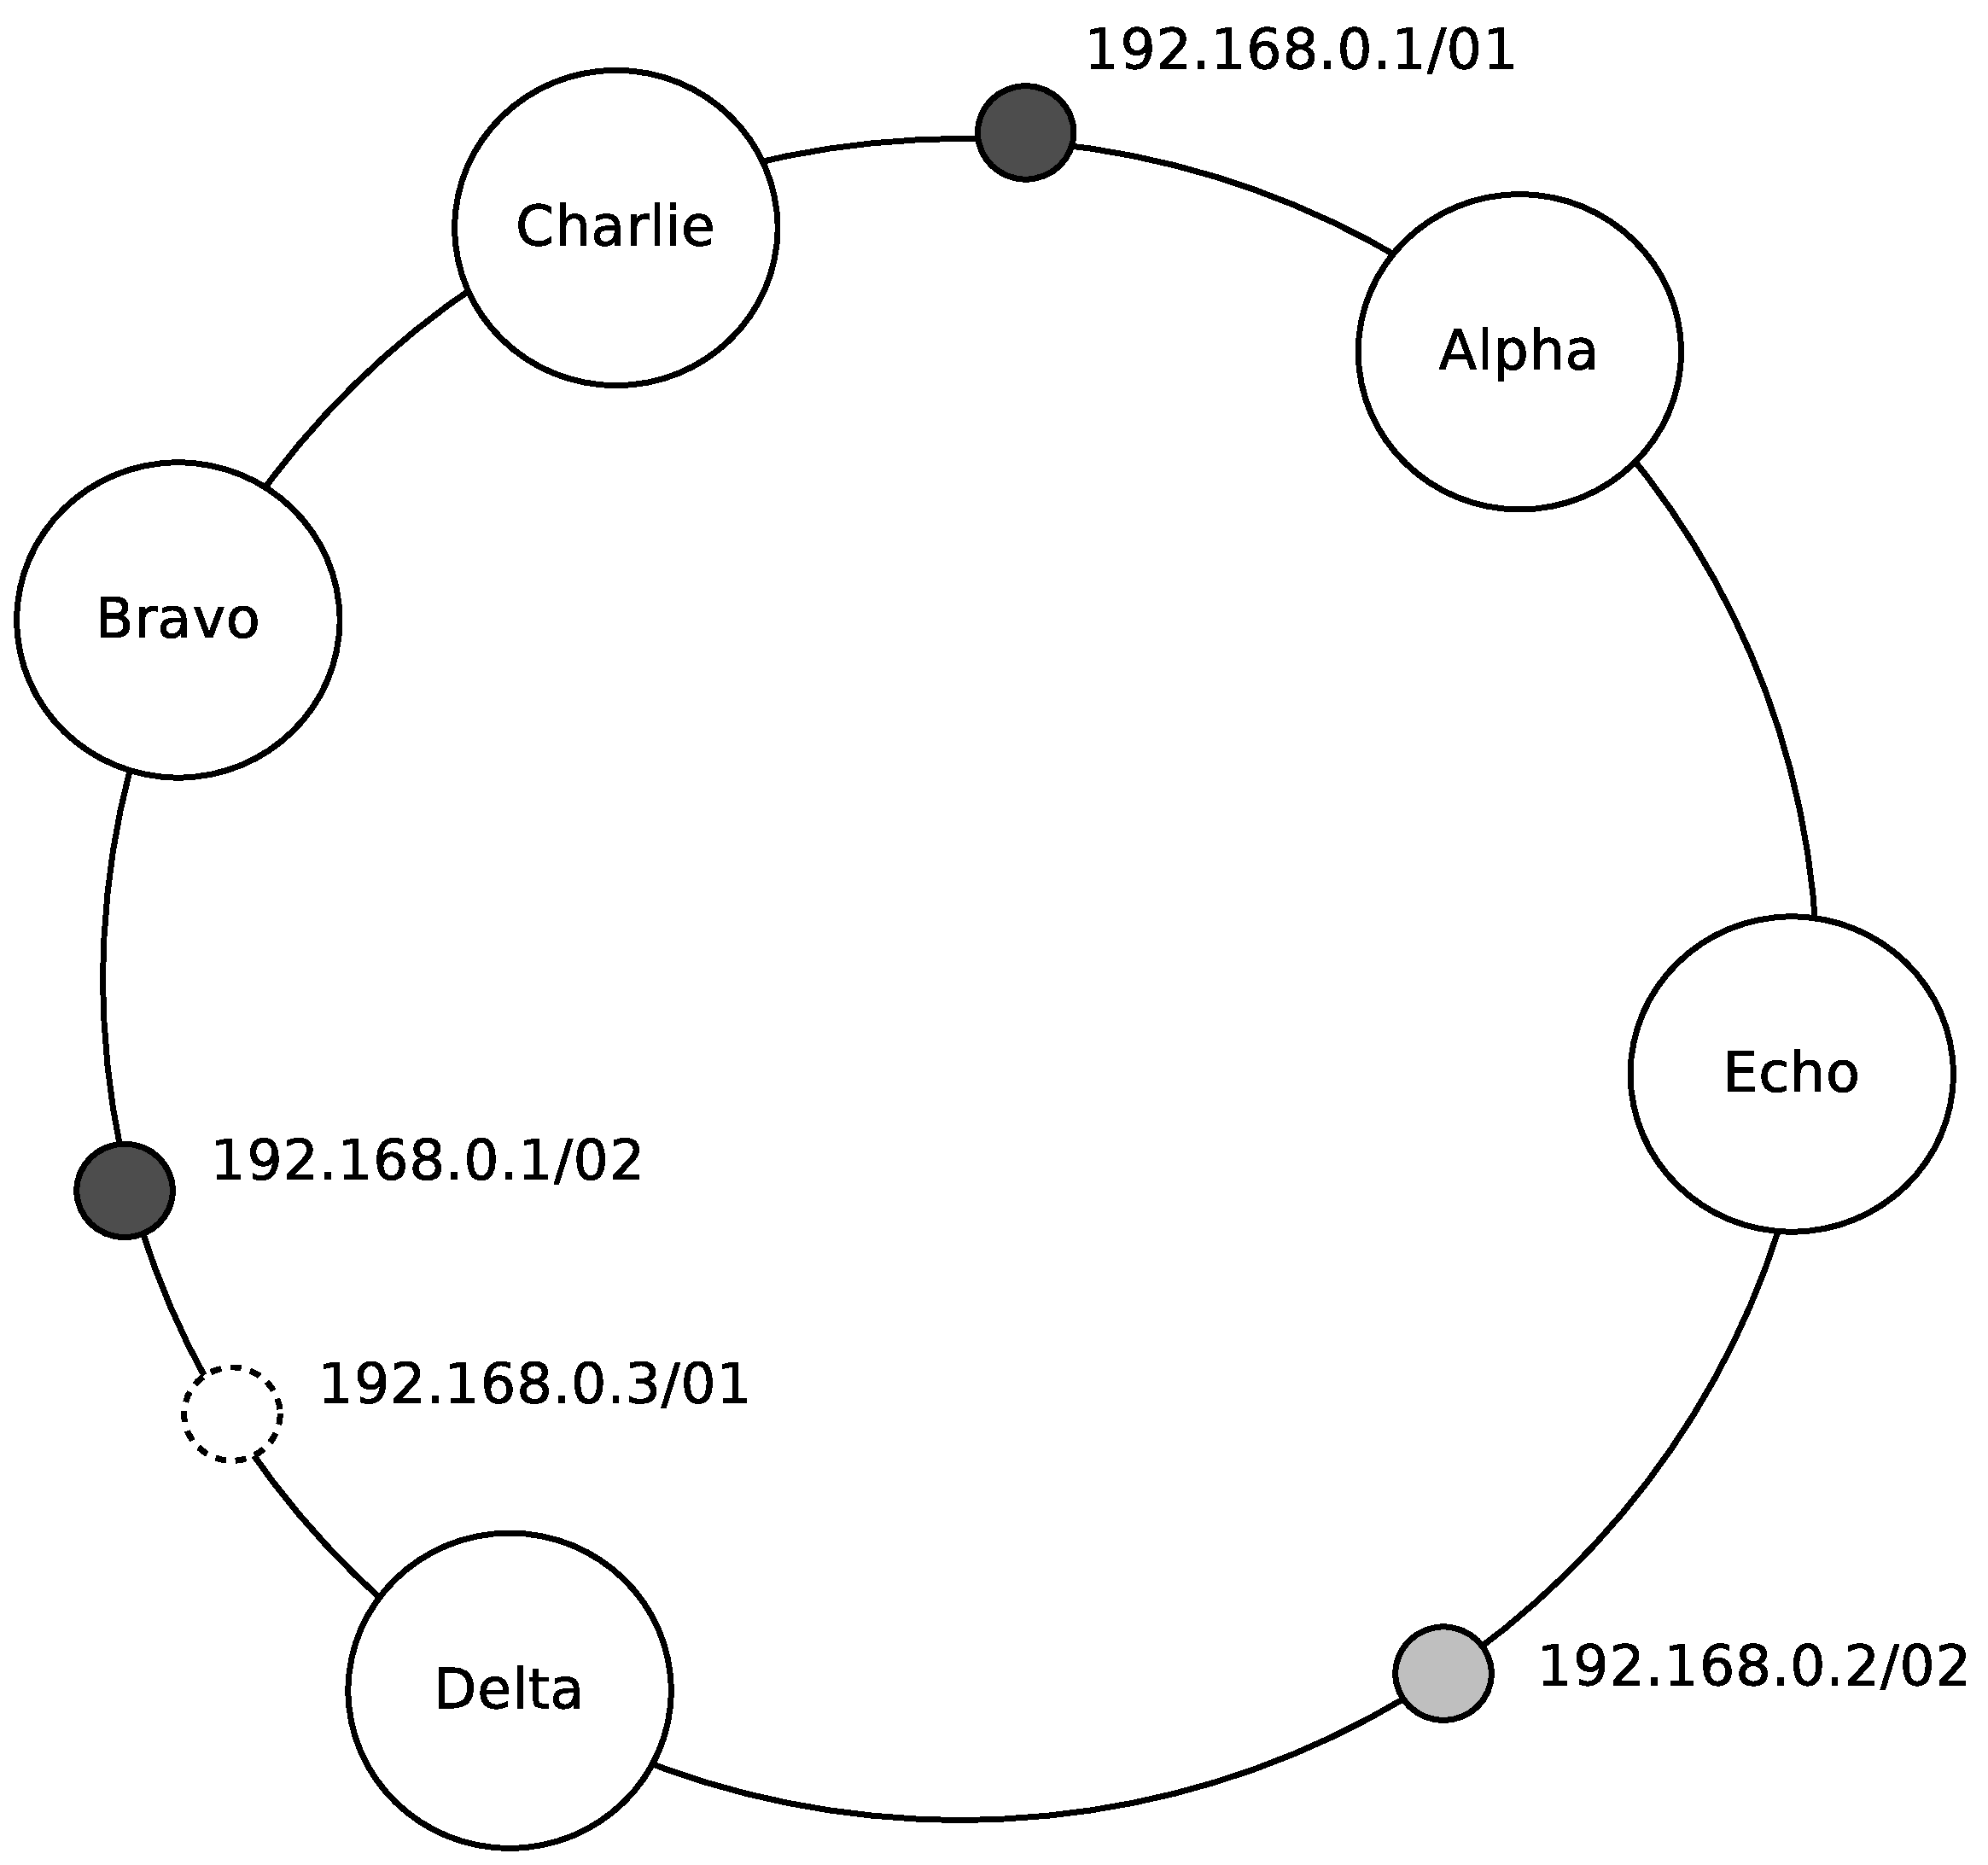
\includegraphics[width=0.8\linewidth]{consistent}
  \caption[一致性哈希算法]{一致性哈希算法。最大的圆环是哈希环。在哈希环上,标
  有字母的大圆代表数据,上面的单词是该数据的索引,图中画出了五个数据。哈希环上
  的小圆代表虚拟结点,旁边标注的字符串是该虚拟结点的标识,同样灰度的小圆对应相
  同的物理结点。系统稳定时有两个物理结点,IP地址为192.168.0.1的物理结点配置了
  两个虚拟结点,用深灰色小圆表示;IP地址为192.168.0.2的物理结点配置了一个虚拟
  结点,用浅灰色小圆表示。对于任何一个数据,其索引的哈希值在哈希环上有唯一的一
  点与之对应。从该点开始,顺着哈希环沿逆时针方向找到M个虚拟结点,这M个结点对应
  的N个不同物理结点即存放该数据的存储服务器,N为数据在系统中的副本数。当系统中
  有新的结点加入,如虚线小圆表示的IP地址为192.168.0.3的存储服务器,假设N等于
  1,需要迁移的数据只有那些索引的哈希值落到从浅灰色虚拟结点到新加入虚拟结点之
  间的劣弧上的数据,这些数据将从深灰色虚拟结点对应的物理结点上移动到新加入的物
  理结点上,即索引值为Delta的数据将从IP地址为192.168.0.1的存储结点上移动到新加
  入的IP地址为192.168.0.3的存储结点上。除此之外,索引的哈希值落在从新加入的虚
  拟结点到浅灰色虚拟结点的优弧上的所有数据都不必做出移动。期望的数据移动量为
  系统中数据总量的(C + 1)分之一,C为结点加入前集群的规模,这也是在保证系统存储
  负载平衡的前提下,任何算法所能达到的数据迁移量下界。此外,一致性哈希算法保证
  了集群中存在结点动态变化时,变化前后系统的存储负载都是均衡的。}
  \label{figure:consistent}
\end{figure}

现在我们有了一个哈希环;对每一个数据的索引求哈希后,在哈希环上都有一点和这个数
据对应;对于集群中的每一台存储服务器,在哈希环上都有若干点与之对应,并且这些点
是随机分布的。在图\ref{figure:consistent}中,最大的圆环是哈希环。在哈希环上,
标有字母的大圆代表数据,上面的单词是该数据的索引。哈希环上的小圆代表虚拟结点,
旁边标注的字符串是该虚拟结点的唯一标识。同样灰度的小圆对应相同的物理结点。那么
如何决定数据的分配和备份呢?一致性哈希算法规定,对于任何一个数据,将哈希函数作
用在它的索引之上,得到的哈希值在哈希环上有唯一一点与之对应。从该点开始,顺着哈
希环沿逆时针方向找到前M个虚拟结点。如果这M个虚拟结点对应N个不同物理结点(N为数
据在整个系统中的副本数,并且显然N不大于M),那么该数据就应当存放在这N个物理结
点上。在图\ref{figure:consistent}中,假设N等于1,那么索引为Alpha的数据应当存放
在IP地址为192.168.0.2的物理结点上,索引为Bravo的数据应当存放在IP地址为
192.168.0.1的物理结点上;如果N等于2,那么图中画出的所有数据都应当在两台服务器
上各存放一个副本。

另一种决定数据在存储服务器之间分配的方法,在实现上比一致性哈希算法简单。首先对
集群中的C台机器从0到C-1依次编号。对于每一个数据,计算其索引的哈希值。由于数据
在计算机中的最终表示是二进制,所以哈希值也可以当成一个整数来处理。将这个整数除
以C,得到的余数即为N等于1时,应当存储该数据的服务器的编号。对于N大于1的情形,
只需要找到编号不小于该余数的连续N台服务器即可。\footnote{如果超过C-1则从0开始
数}这种\emph{除留余数法}与一致性哈希算法相比,思路更加直观,实现也方便,对于集
群结点固定的系统,不失为一种理想的解决方案。

但是在大型的数据中心里,集群规模一般为几千台甚至更多的服务器,结点故障不是偶尔
发生,而是可能一直存在。这要求有一种算法能够应对结点的动态加入和移出,将这种变
化造成的数据迁移量降至最低。对于除留余数法,假设集群中总数据量为D,当有一个新
存储结点加入原本规模为C的集群,那么需要迁移的数据量由公式\ref{equation:modula}
计算得:
\begin{equation}\label{equation:modula}
(\frac{D}{C} - \frac{D}{C - 1}) * (1 + 2 + \dots + (C - 1)) = \frac{D}{2}
\end{equation}
也就是说,当有一个结点动态加入集群时,平均有一半的数据要从原存储服务器移动到另
一台服务器。结点移出集群是加入的逆过程,所以当有一个结点因为故障而不再正常运转
时,平均有一半的数据将发生转移。当结点故障异常频繁时,这种数据迁移规模将耗费大
量的网络带宽和硬盘读写资源,对分布式存储系统将是一个极大的负担。

再回到一致性哈希算法。假设系统稳定后有一个新的存储服务器加入了集群,并且它设置
了一个虚拟结点,如图\ref{figure:consistent}中虚线小圆所示。当N等于1时,需要迁
移的数据只有那些索引的哈希值落到从浅灰色虚拟结点到新加入虚拟结点之间的劣弧上的
数据,这些数据将从深灰色虚拟结点对应的物理结点上移动到新加入的物理结点上,即索
引值为Delta的数据将从IP地址为192.168.0.1的存储结点上移动到新加入的IP地址为
192.168.0.3的存储结点上。除此之外,索引的哈希值落在从新加入的虚拟结点到浅灰色
虚拟结点的优弧上的所有数据都不必做出移动。当N大于1时,情况与之类似,请读者以图
\ref{figure:consistent}为例自行判断哪些数据应该做出移动。那么系统中需要移动的
数据总量是多少呢?考虑结点加入的逆过程,即有一个结点离开集群,需要移动的所有数
据就是这个结点原先负责存储的所有数据。由于每个物理结点对应很多的虚拟结点,而这
些虚拟结点又是随机分布的,因此在结点离开集群之前,数据在集群中的分布是近似平均
的。也就是说,规模为C的集群,一个结点动态离开带来的数据迁移量是$\frac{D}{C}$,
一个结点动态加入造成的数据迁移量是$\frac{D}{C + 1}$。显然这两个数值是在保证系
统存储负载均衡的性质下,数据迁移量的下界。因而当结点动态移入和移出系统时,一致
性哈希算法在数据迁移量方面是最优的算法,并且达到了理论下界。一致性哈希算法的另
一个优点是在集群中结点动态变化时,它仍然保持了系统存储负载均衡的性质。前面已经
分析过,当系统稳定时,一致性哈希算法保证了存储负载均衡。当某个物理结点离开集群
后,原先那些由它某个虚拟结点负责的数据,将被这个虚拟结点按顺时针方向看的下一个
虚拟结点所承担。由于物理结点的所有虚拟结点是随机分布的,那么当一个物理结点对应
足够多的虚拟结点时,这些被选中的虚拟结点将以相同的数目对应全部的物理结点。换句
话说,原先由那个离开的物理结点存储的数据将被平均分成若干份,集群中其余的每个物
理结点将得到相同的份数,所以得到的数据总量也相同。因此,一致性哈希算法保证了集
群中存在结点动态变化时,变化前后系统的存储负载都是均衡的。

分布式二级哈希表的配置服务器实现了一致性哈希算法。开源项目libconhash是一个用标
准C语言写就的,能在Windows和Linux平台下运行的一致性哈希算法实现。但是它不支持
在系统中进行数据备份,并且其中一些功能的实现策略不适合分布式二级哈希表。因此我
在原工程的框架下重写了部分代码,添加了诸多功能,比如使得系统可以支持数据备份,
最终将其成功移植到分布式二级哈希表系统中来。

在分布式二级哈希表中,由于系统设计不考虑结点动态加入和离开的情形,因此配置服务
器通过读取配置文件获取集群中所有存储服务器的主机名或IP地址。由于集群中各存储结
点是同构的,因此直接设定每个物理结点对应1024个虚拟结点。哈希函数选用128位MD5哈
希\cite{rivest1992rfc1321},保证了虚拟结点在哈希环上的随机分布性质。

实现一致性哈希的另一个关键点是如何在哈希环上快速找到顺时针方向下一个虚拟结点。
由于C语言的标准库中不具有像Java语言中HashMap那样的数据结构可以直接调用实现此功
能的接口函数,在分布式二级哈希表中,这个问题通过自行实现了一棵红黑树
\footnote{http://en.wikipedia.org/wiki/Red-black\_tree}来解决。红黑树是一种平
衡二叉搜索树,它具有以下性质:
\begin{enumerate}
  \item 结点被涂以红色或者黑色。
  \item 根结点被涂以黑色。
  \item 所有叶结点被涂以黑色。
  \item 所有红色结点的左右子结点都被涂以黑色。
  \item 给定一个结点,从这个结点开始到它任何一个后代叶结点的所有路径包含相同数
  目的黑色结点。
\end{enumerate}
这些性质保证了红黑树是一棵基本平衡的二叉树,在它上面进行搜索的最差时间复杂度为
O(log(N)),其中N为红黑树中结点的个数。在分布式二级哈希表中,所有的虚拟结点都有
一个在红黑树中的叶子结点与之对应,排序依据就是这个虚拟结点的标识字符串的MD5
值。当我们需要查看一个某个数据存储在哪些物理结点上时,就把这个数据的索引取MD5
值,再拿这个值在红黑树中去搜索,找到第一个哈希值不小于这个值的虚拟结点,再从这
个虚拟结点的哈希值开始,往后找N - 1个哈希值严格增大,并且对应不同物理结点的虚
拟结点。如果在这个过程中需要找比某个值大的虚拟结点,但是这个值比红黑树中最大的
哈希值还大,那么直接返回哈希值最小的那个虚拟结点。给定索引确定数据所在存储服务
器的IP地址的函数伪代码如下:
\begin{code}
  FUNC getIpsByKey(IN string key, IN int N, OUT IP[] ips)
  {
    GLOBE RBTREE rbtree;
    VAR VNODE vnode, start;

    vnode = rbtree.geq( MD5(key) );
    ips[0] = vnode.node.ip;
    start = vnode;
    for i from 1 to (N - 1)
    {
1:    vnode = rbtree.ge( vnode.hash );
      if ( vnode == start ) ERROR;
      for j from 0 to i - 1
      {
        if ( ips[j] == vnode.node.ip ) goto 1;
      }
      ips[i] = vnode.node.ip;
    }
  }
\end{code}
前面我们说到在红黑树中搜索的时间复杂度为O(log(N)),其中N为树中结点总个数。在分
布式二级哈希表的一致性哈希实现中,红黑树中的结点数就是系统中虚拟结点的总数。在
第\ref{section:assumption}节中的一个假设是系统的典型规模为50台存储服务器,按照
上文提到的每个物理结点配置1024个虚拟结点计算,一次查询需要花费的时间规模与处理
器进行16次运算相当,因此用红黑树实现一致性哈希具有很高的查询效率。

此外,之前在原理介绍中提到的数据索引,在分布式二级哈希表的实现中,指的是blob的
bucketID。也就是说,同一个桶中的blob将存储在相同的服务器上。一致性哈希算法对于
数据的分配粒度是相对于桶的,它不能区分同一个桶中不同的blob。在这种情况下,集群
的存储负载平衡是由另一个假设保证的。即我们假设单个blob较小,但是blob和桶的个数
很多。如果我们将桶中所有blob的大小求和作为桶的大小,那么虽然桶的大小可能差异很
大,但是由于每个物理结点都存储了很多的桶,而且这些桶是随机分配的,那么当桶的数
目足够多时,每个物理结点的总存储量是近似相同的。

\subsection{远程过程调用}
除了一致性哈希算法,配置服务还包含另一个重要模块,即远程过程调用模块。在分布式
二级哈希表中,客户端通过远程过程调用从配置服务器获取某个数据所在的目标存储服务
器的IP地址。

远程过程调用是一种客户端和服务器交互的技术,它使得客户端程序可以调用执行在远端
服务器上的一段程序,而调用方法就好像在执行本地的函数一样,不必关心客户端和服务
器的网络交互,以及其他实现细节。分布式二级哈希表采用ONC RPC
\footnote{http://en.wikipedia.org/wiki/ONC\_RPC}标准规定的远程过程调用协议,代
码执行流如图\ref{figure:oncrpc}所示。客户端执行clnt\_call系统调用,并将参数按
照本地函数调用的方式压栈。clnt\_call从中提取出目标服务器例程的信息,并将该例程
需要的参数按照事先定义的方式打包,然后通过TCP或UDP协议将参数发送至指定服务器。
目标服务器事先已经注册了一段例程,并监听ONC RPC使用的默认端口111。一旦收到客户
端发来的打包数据,按照事先定义的方式从中提取出参数,并传递给服务器例程。接着服
务器例程在用户态执行,执行完毕后,进入内核态,由操作系统将返回值按照事先约定的
方式打包,再依照相同的传输层协议,通过刚才建立的连接,将打包后的返回值传回客户
端。至此,此次远程过程调用服务器端的工作完成,服务器端准备应答下一个请求。客户
端收到服务器发送来的打包数据,按照事先约定的方式从中提取出返回值。然后
clnt\_call系统调用返回,将远程过程调用的返回值传递给用户态的客户端主程序,本次
远程过程调用执行完毕。
\begin{figure}
  \centering
  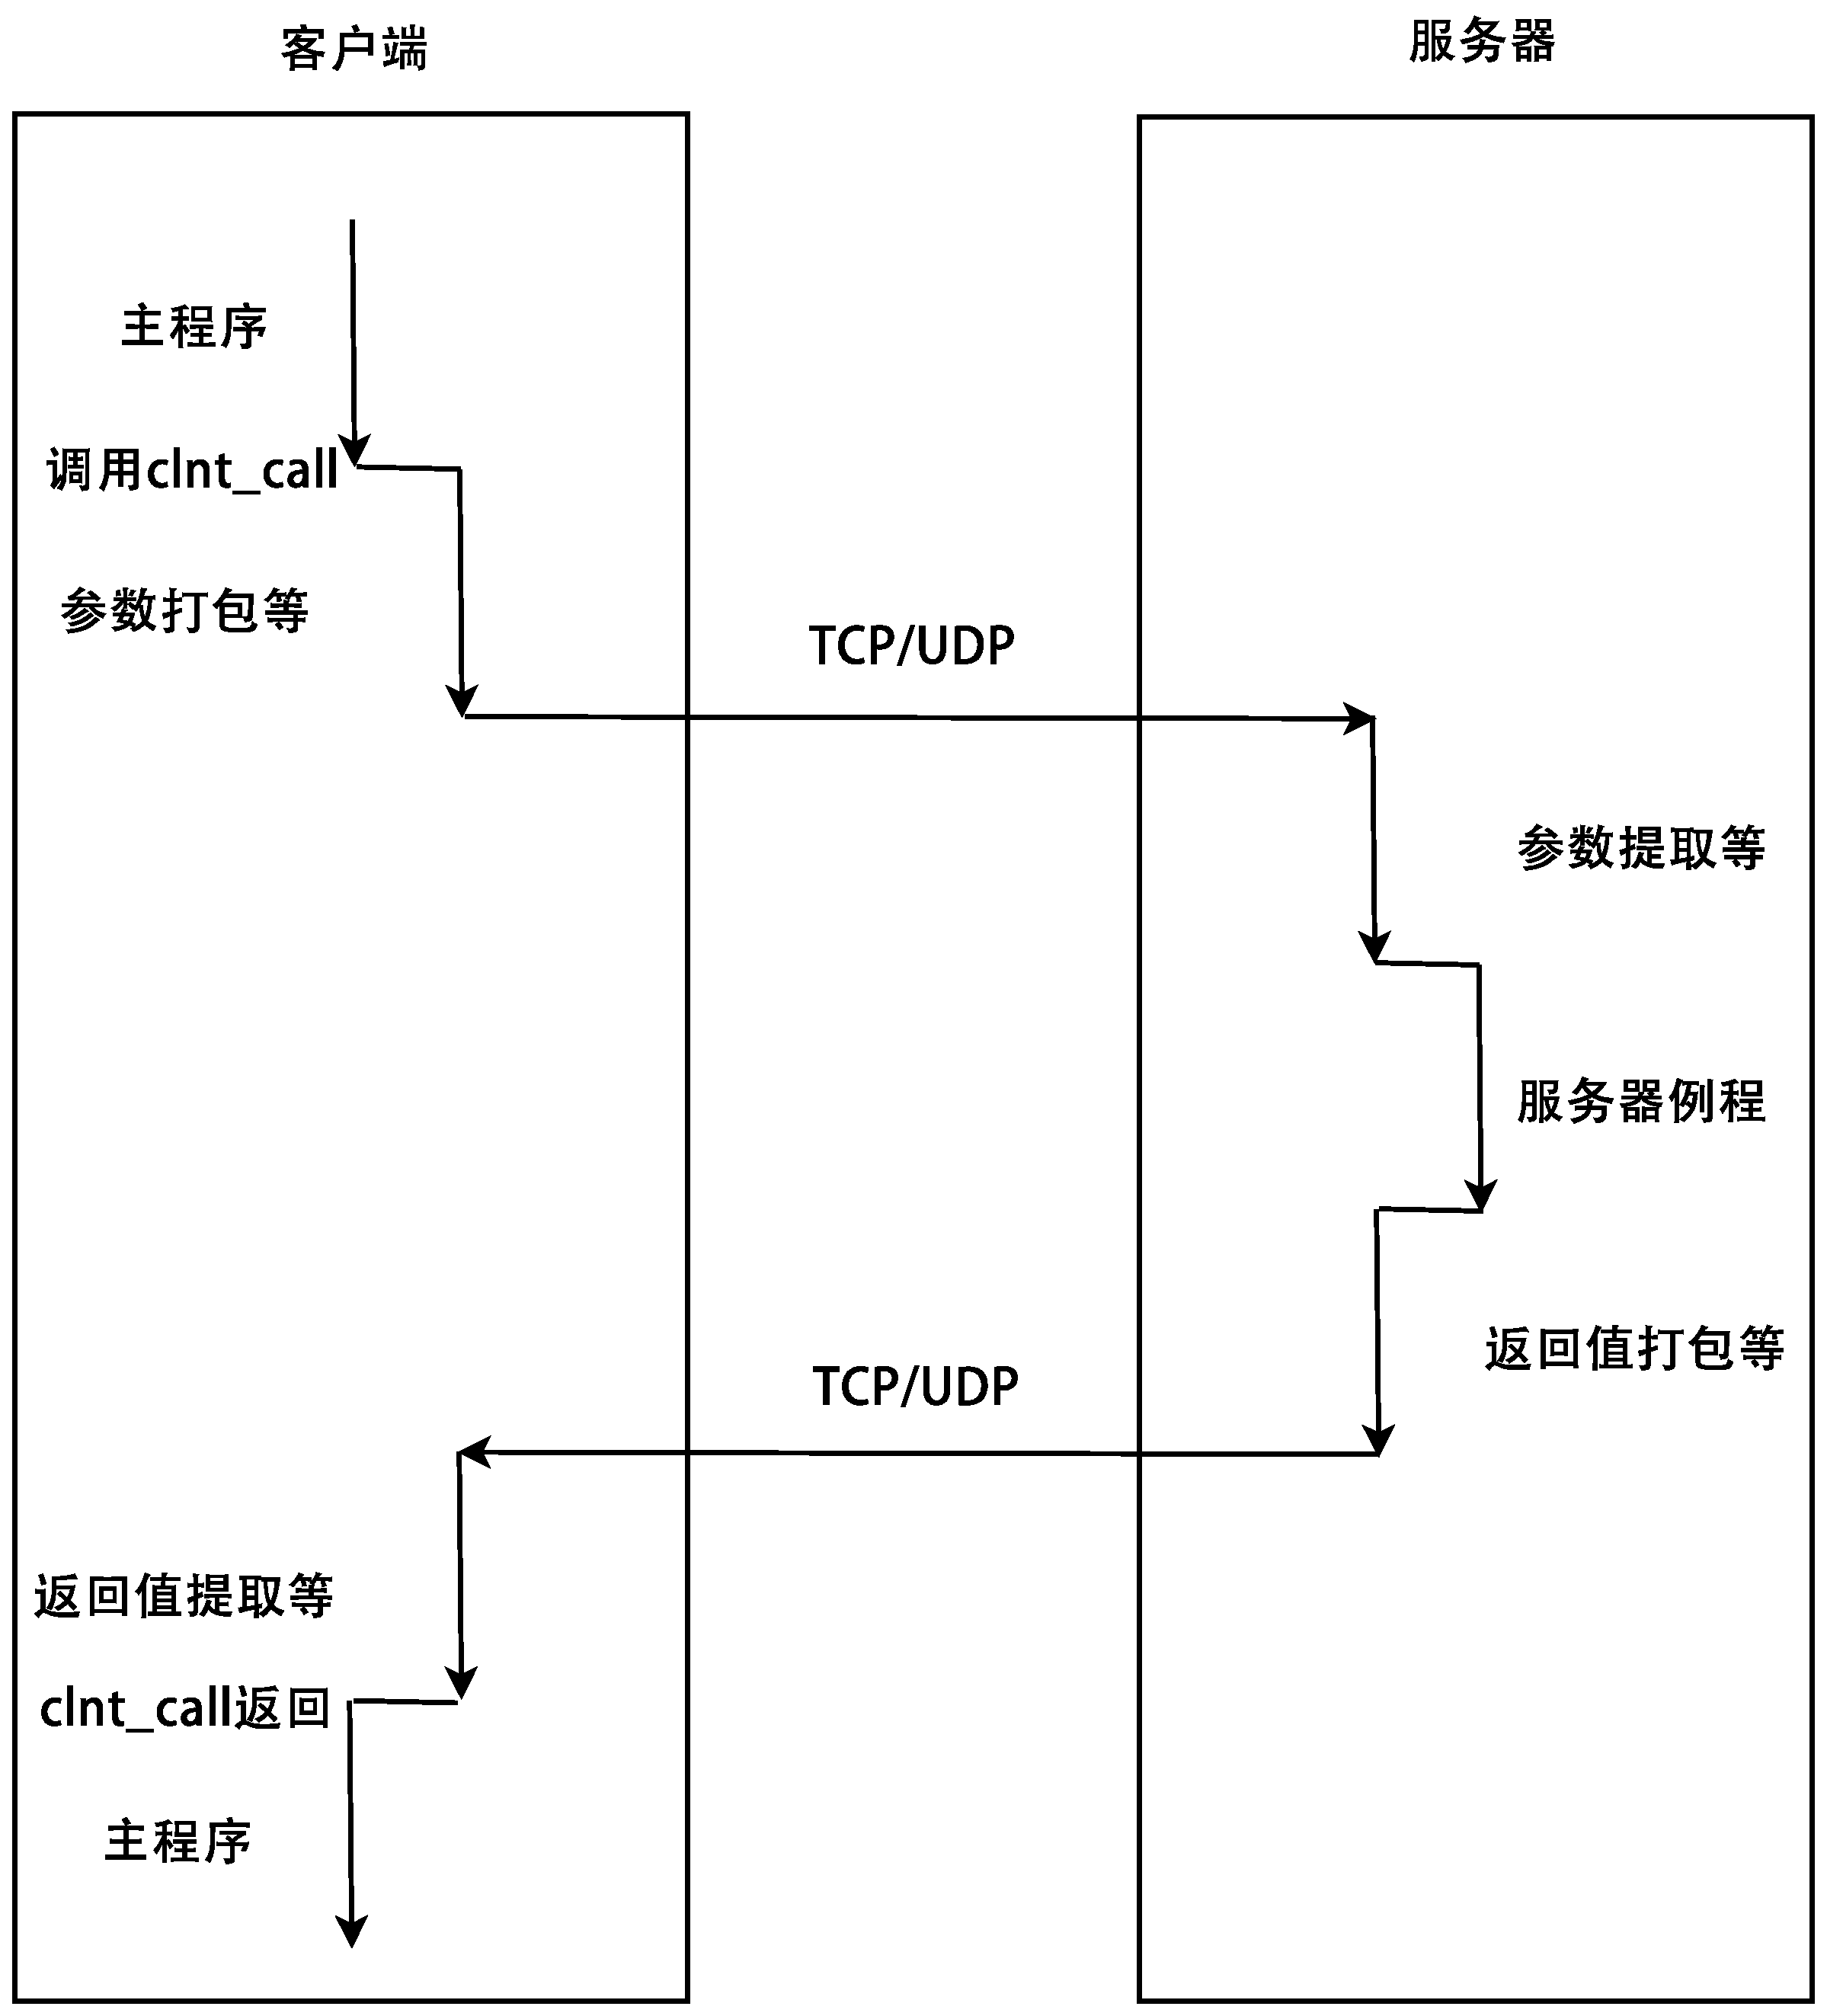
\includegraphics[width=1.0\linewidth]{oncrpc}
  \caption[ONC RPC代码执行流]{ONC RPC代码执行流。客户端用户态主程序执行
  clnt\_call系统调用。clnt\_call将服务器目标例程需要的参数按照事先定义的方式打
  包,然后通过TCP或UDP协议将打包数据发送至指定服务器。目标服务器事先已经注册了
  一段例程,并监听ONC RPC使用的默认端口111。收到客户端发来的打包数据后按照事先
  定义的方式从中提取出参数,并传递给用户态服务器例程。服务器例程执行完毕后,进
  入内核态,由操作系统将返回值按照事先约定的方式打包,再通过刚才建立的连接将打
  包后的返回值传回客户端。至此,此次远程过程调用服务器端工作完成,端准备应答下
  一个请求。客户端收到服务器发送来的数据,按照事先约定的方式从中提取返回值。然
  后clnt\_call返回,将远程过程调用的返回值传递给用户态的客户端主程序,本次远程
  过程调用执行完毕。}
  \label{figure:oncrpc}
\end{figure}

远程过程调用这种客户端和服务器的交互机制,简化了程序员的编程,其中,参数和返回
值的打包,数据在客户端和服务器之间的可靠性传输等工作均由系统来实现。但是,上述
代码执行流程对于纯粹写应用的程序员仍然略显复杂,比如,程序员需要\emph{告知}系
统如何对数据进行打包和提取,需要初始化网络参数等。为了进一步简化程序员编程,使
程序员将主要精力放在将要实现的功能上,而不是远程过程调用本身的实现上,编程工具
rpcgen\footnote{http://en.wikipedia.org/wiki/Rpcgen}应运而生。程序员只需要书写
一个简单的配置文件,声明服务器例程的原型,以及各参数和返回值的数据结构,rpcgen
就能据此产生出服务器和客户端将要用到的全部C代码。程序员只需要在服务器端例程的
框架里填入具体实现,再将客户端代码和服务器端代码分别编译,便实现了远程过程调
用。比如,在分布式二级哈希表中,客户端通过远程过程调用,给定一个索引,从配置服
务器得到具备这个索引的数据所在的存储服务器的IP地址。那么rpcgen的配置文件
cfgsrv.x内容非常简单:
\begin{code}
typedef u_int ips<>;

program CFGSRVPROG {
  version CFGSRVVERS {
    ips GET_HOSTS_BY_KEY(string) = 1;
  } = 1;
} = 1;
\end{code}
其中指定了服务器端例程的原型。参数只有一个,即字符串类型的索引值。返回值是无符
号类型整数的可变长度数组,其中每个元素是一个目标存储服务器的IP地址。rpcgen据此
生成了四个文件:
\begin{enumerate}
  \item cfgsrv.h: 基本的声明文件。编译客户端和服务器端程序时都需要引入此头文
  件。
  \item cfgsvr\_clnt.c: 客户端辅助文件,以实现远程过程调用机制,其中只定义了一
  个函数get\_hosts\_by\_key\_1。客户端主程序调用这个本地函数,就能从配置服务器
  获取目标存储服务器的IP地址。
  \item cfgsrv\_svc.c: 服务器端辅助文件,以实现远程过程调用机制。
  \item cfgsrv\_xdr.c: 服务器端例程的参数和返回值打包程序。
\end{enumerate}
为了完成远程过程调用机制,服务器端还需要实现cfgsrv.h中声明的
get\_hosts\_by\_key\_1和get\_hosts\_by\_key\_1\_svc两个函数。其中第一个函数是
服务器端真正完成通过索引获取目标存储服务器IP地址的例程,可以调用第
\ref{subsection:consistent}小节介绍的一致性哈希算法的实现函数。第二个函数只是
对第一个函数的包装。之后通过rpcgen -m命令可以得到服务器端初始化远程过程调用的
代码。至此,将上述文件合理编译,即可得到实现了远程过程调用的服务器和客户端模
块。

远程过程调用简化了客户端和服务器端实现通信的机制。如果不使用远程过程调用,一种
实现方式是直接在客户端和服务器端建立TCP/UDP连接,再按照自定义的协议传送数据。
在第\ref{section:assumption}实验假设中提到分布式二级哈希表平均每台服务器每秒处
理的请求数不小于50,平均响应时间为百毫秒数量级,这说明客户端一直会发起大量的请
求。如果每一个请求完成之后都关闭socket连接,下个请求到来时再重新建立连接,那么
创建socket和回收资源的系统开销将会非常大,严重影响系统运行性能。这要求每个客户
端和配置服务器的socket连接一直持续,直到客户端程序全部运行结束。基于这个前提,
由于要保证系统的平均响应时间和吞吐量,请求必须设定为异步的,而不能像同步系统那
样将请求放置在一个队列里,在上一个请求结束之后再处理下一个请求。因此,请求的返
回顺序可能和发起顺序不同,客户端可能先收到后发出的请求的返回值,再收到先发出的
请求的返回值。在同一个socket连接中,客户端需要为每个请求附上一个唯一的流水号,
服务器则要为返回值贴上相同的流水号。另一方面,在编程实现上,异步请求也较同步请
求更为复杂,容易出错且不易调试。如果维护返回值和请求的对应关系,以及请求的异步
化都由远程过程调用的框架来完成,那么对于程序员来说,客户端的每次请求就是对本地
函数的一次调用,不必过多考虑上述实现细节。

\section{客户端}\label{section:client}
在第\ref{chapter:architecture}章中曾介绍过,分布式二级哈希表中的客户端是一个独
立的模块,是分布式二级哈希表的一个函数库,上层应用需要将这些代码编译到可执行文
件中去。客户端直接从配置服务器拿到目标存储服务器的IP地址,再与这些服务器进行通
信,执行操作,并将返回值传递给上层应用。这样,完成一次操作总共需要进行两次网络
通信。第一次是客户端通过远程过程调用从配置服务器拿到路由信息,第二次是客户端将
请求发送给具体的存储结点,得到返回值。这种决策的缺点是上层应用需要嵌入分布式二
级哈希表的标准C代码,降低了分布式二级哈希表的易用性和通用性。另一种不需要嵌入
系统框架代码的解决方案是,让客户端直接与某一台入口服务器按照某种协议进行通信,
再由这台入口服务器完成客户端的功能。这样入口服务器和客户端之间还要多进行一次网
络通信,势必增加请求的平均响应时间,并且消耗网络带宽。由于分布式二级哈希表更在
意系统的运行效率,而且上层应用是由我们自己搭建的,因此最终我选用了第一种方案来
实现客户端。

客户端采用了分层结构,如图\ref{figure:client}所示。最上层是接口层,对分布式二
进制哈希表提供的各项功能做出了最外层的包装,为上层应用提供调用接口。接口层通过
调用路由层的相应函数,将上层应用的请求向下面传递。路由层收到请求后,首先通过远
程过程调用从配置服务器得到数据所在的存储服务器的IP地址,然后按照Redis规定的交
互协议构建命令闭包,将其丢进线程池的任务队列中。最后在规定的时限内检查该命令闭
包的执行结果,并将返回值传递给上层函数。为了提高系统的性能,我在路由层的下面实
现了一个线程池。该线程池有一个任务队列,其中的元素是Redis命令闭包,包含一条
Redis命令的全部信息。线程池会自动执行队列中的任务,并将返回值填入命令闭包。这
样路由层就可以方便的将上层应用的请求转化为Redis命令,将构建好的命令闭包丢进线
程池的任务队列。在线程池之下是通信层,主要实现了Redis规定的交互协议,与存储服
务器上Redis服务器进程进行交互,执行各种命令并获取返回值。总体来说,除了接口
层,分布式二级哈希表中的每一层都通过调用下层的某一函数,实现请求逐级向下传递。
而下层执行完该函数之后,通过函数返回将结果数据传递回上一层。横向来看,路由层和
配置服务器之间有一次网络通信,获取数据所在存储服务器的IP地址;通信层和存储服务
器之间也有一次网络通信,执行真正的Redis命令并取得返回值。两层之间的线程池实现
了请求的异步化,充分利用了网络带宽,大大提高了系统的运行效率。下面我将详细介绍
分布式二级哈希表客户端的各个子模块。
\begin{figure}[htb]
  \centering
  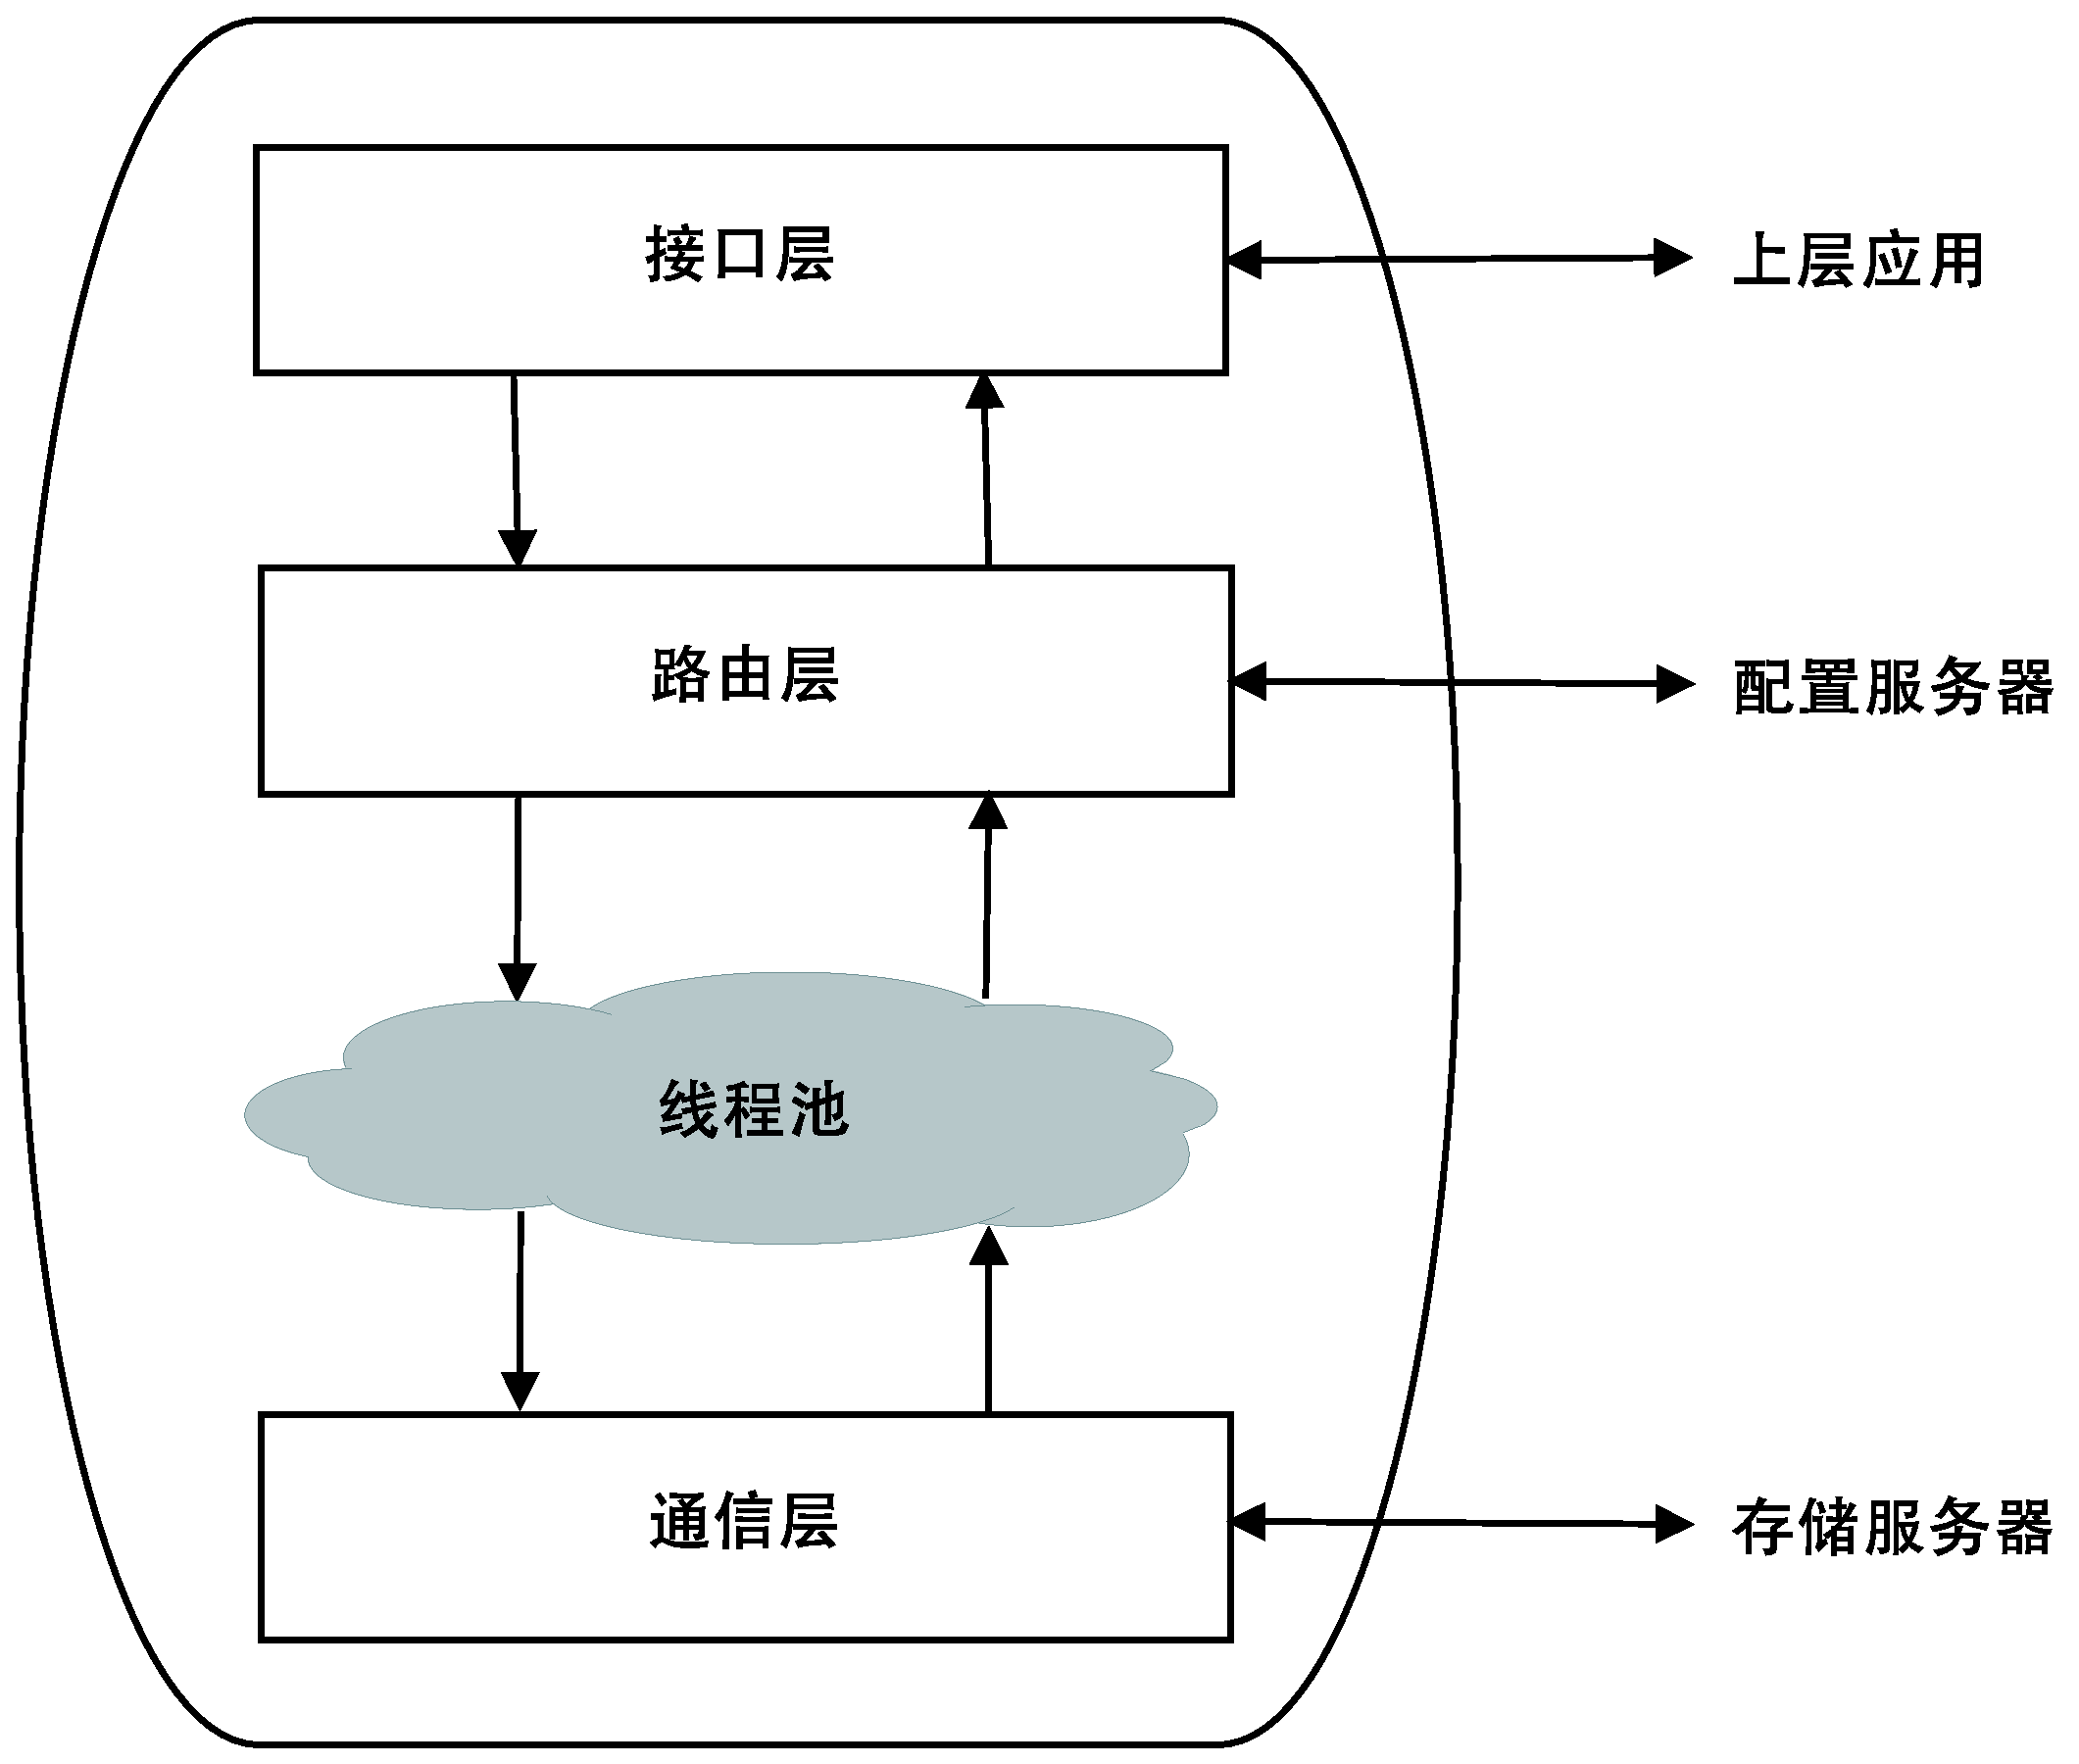
\includegraphics[width=0.8\linewidth]{client}
  \caption[分布式二级哈希表客户端]{分布式二级哈希表客户端分层结构。最上层是接
  口层,对分布式二进制哈希表提供的各项功能做出了最外层的包装,为上层应用提供调
  用接口。接口层之下是路由层,通过远程过程调用从配置服务器得到数据所在的存储服
  务器的IP地址,然后按照Redis规定的交互协议构建命令闭包,将其丢进线程池的任务
  队列,再异步检查其执行结果。线程池会自动执行任务队列中的命令,并将返回值填回
  命令闭包。最下层的通信层按照Redis规定的协议与存储服务器上的Redis服务器进程进
  行通信,将指令发送给存储服务器并取得返回值。纵向来看,请求和参数由上而下逐级
  传递,返回值则由下而上逐级返回。横向来看,路由层从配置服务器获取存储服务器的
  IP地址有一次网络通信,通信层和目标存储服务器之间还有一次网络通信。}
  \label{figure:client}
\end{figure}

\subsection{接口层}
接口层对分布式二级哈希表实现的各项功能做了最外层的包装,将其呈现给上层应用。在
接口层的头文件api.h里声明了可供上层应用调用的所有函数,具体功能详见表
\ref{table:api}。数据的返回是通过上层应用在调用接口函数时,传入指针实现的。调
用者负责为该指针申请足够的空间,接口层则会在从该指针所指地址开始填入返回的数
据,如果该函数需要返回数据的话。每个函数的返回值则标识了该请求是否成功执行。在
上层应用调用任何接口函数之前,还需要调用接口层的初始化函数。初始化函数将该层需
要用到的模块和全局变量等资源进行初始化,并调用下层的初始化函数。与此类似,客户
端所有请求执行完成后,调用接口层的终结函数。

\subsection{路由层}
回顾一下,在第\ref{chapter:architecture}章中我说明了为什么同一个数据在分布式二
进制哈希表中要存储多份,以及不同副本之间的数据保证了弱一致性,即不同副本之间的
数据并不是时刻保证相同的,但读操作总能读取到对该数据的最近一次写操作结果。在分
布式二级哈希表中,数据的弱一致性通过\emph{$R+W>N$语义}实现。

\subsubsection{$R+W>N$语义}
$R+W>N$语义是分布式系统中保证数据弱一致性的经典算法之一,它指的是如下算法。在
数据有N个副本的分布式系统中,每个读写操作都要对N个副本同时进行。对于写操作,只
要在至少R个副本上成功写入了,即认为该写操作成功了。对于读操作,只要读出了至少W
个副本上的数据,那么其中至少有一份数据是最新写入的数据。其中,R和W的数值人为设
定,但必须满足二者之和大于N。原理的正确性是显然的。

相比与维护数据的强一致性,$R+W>N$语义的优点如下:
\begin{enumerate}
  \item $R+W>N$语义提高了系统的操作成功率,降低了响应延迟,大大提高了系统性
  能。强一致性系统中,如果由于网络阻塞或者其他原因,在一个副本上写操作执行失败
  了,那么整个写操作就执行失败了。即便能够执行成功,这次写操作的响应时间也取决
  于N个操作中最慢的那个。而在$R+W>N$语义中,写操作取决于这N个操作中第R快的那个
  操作。由于R小于N,平均响应时间必定减小。另一方面,由于只要在R副本上成功写入
  了数据,即宣告该写操作成功执行了,系统的操作成功率必定增加。
  \item $R+W>N$语义可以针对不同的应用需求,对系统的性能作出调整。R越大,系统对
  于读操作的响应时间越小,数据的一致性越强;W越小,系统对于写操作的响应时间越
  小。
  \item $R+W>N$语义可以简化系统实现。在强一致性系统中,如果某个操作失败,需要
  将系统恢复到这N个子操作进行之前的状态。也就是说,即便N个写入操作中的某些成功
  了,也要将数据恢复到写入之前的数值。这将大大增加系统的实现难度,降低系统的运
  行效率。\cite{fox1997cluster}而在弱一致性系统里,操作的成功率很高,因此读操
  作总能读到最新写入的数据。
\end{enumerate}
回忆第\ref{section:assumption}节,我们要求系统在饱和运转时,操作成功率大于
99.999\%,而平均响应时间在百毫秒数量级,如此严苛的条件必然要通过采用$R+W>N$语
义来满足。

在分布式二级哈希表中,路由层针对每一个请求,将其转化为一条Redis命令,构建出N个
命令闭包后丢入线程池的任务队列。线程池对任务的执行是异步的,路由层需要在一定的
时限内去检查执行情况,并将最终结果返回给接口层。关于命令闭包、线程池和异步结果
提取将在稍后第\ref{subsection:threadpool}小节详细介绍。

与强一致性分布式存储系统相比,$R+W>N$语义带来了系统性能的显著提升,但是延长了
读操作的平均响应时间。原先N个读操作只要有一个成功执行了,即可以直接返回其结
果,现在不仅要等R个结果,而且由于数据是弱一致性的,系统只能保证这R个结果中至少
\emph{有一个}是最新版本的数据,但可能不都是最新版本的数据。这要求系统能够通过
某种机制从中挑选出最新版本的数据,这一过程称为版本冲突解决。

\subsubsection{版本冲突解决}
在仅保证数据弱一致性分布式系统中,$R+W>N$语义确保读到的R个版本的数据中有一份是
最新写入的,但这R份数据可能不全是最新的版本。分布式系统领域里一般通过如下方式
解决这个问题:在写入时为数据添加版本信息,在读数据时根据版本信息判断它们的时序
关系,选取最新的数据。添加版本信息的最常用方法是向量时钟
\cite{lamport1978time},比如在Dynamo\cite{hastorun2007dynamo}的实现中就使用了
这种方法。但是向量时钟不能解决所有的版本冲突问题,当有无法解决的冲突时,Dynamo
将所有版本的数据返回给上层应用,由他们自己来解决。

分布式二级哈希表的设计不允许有多个版本的数据反馈给上层应用。由于版本冲突是异步
分布式系统的固有性质,不可能通过任何算法彻底解决。而且系统存储的是没有任何子结
构的二进制数据块,不可能有任何智能的算法将冲突的数据综合出一个新的版本。因此当
有不可解决的数据冲突发生时,分布式二级哈希表必然只能从中随机选取一个版本的数据
作为返回值。另一方面,尽管为了降低写操作的响应时间,N个副本中只要有W个成功写入
了数据,该操作就成功返回了,但是在不发生错误的情况下,这N个副本上的数据最终都
会被更新。此外,如果采用向量时钟标记数据版本,那么在执行写入操作时,必然要附加
一次读取操作取得数据的版本信息,这必然会增加写入操作的平均响应时间。第
\ref{section:assumption}节提到,容许个别情况下读到不是最近一次写入的数据。综合
以上考虑,为了简化系统设计和实现,最终我决定直接从读到的R个副本中随机选取一份
数据作为返回值。为了减少这种策略可能带来的风险,对于blob的读写操作,设定
$(N, W, R) = (3, 2, 2)$,这是主流分布式存储系统的一般配置方法;对于桶和blob的
删除操作,以及检测指定桶和blob是否存在的操作,设定$(N, W, R) = (3, 3, 1)$,即
删除操作要求在所有副本上全部成功执行,而只要有一个副本上还残留有数据,即认为该
数据存在。由于删除操作和检测操作的出现频率读写操作低很多,这种配置在对系统性能
造成可以忽略的影响的前提下,很大程度上提高了操作的语义正确性。

\subsection{线程池}\label{subsection:threadpool}
$R+W>N$语义通过减小写操作的响应时间来提高系统的性能,具体来说,由原本需要等待N
个副本上操作全部完成,改进为只需要等待至少R个副本上成功写入了数据即可。系统满
足这个性质的前提是,在N个副本上的操作是并行执行的,其中每个操作包括客户端将命
令请求发送至存储服务器,存储服务器在本地执行相应操作,存储服务器将操作的返回值
发送回客户端。为了实现操作的并行执行,必然要用到多线程或者多进程技术。进程间通
信需要用到特定的技术
\footnote{http://en.wikipedia.org/wiki/Inter-process\_communication},相比起
来,同一进程下的线程共享内存地址空间、文件描述符等系统资源,不同线程之间交换数
据几乎不用引入额外的系统开销。另一方面,线程比进程更轻量级,其创建和资源回收比
线程的开销要小很多。综合以上两点考虑,我最终选择多线程技术实现操作的并行化。在
第\ref{section:assumption}节中介绍过,在系统饱和运转的情况下,单位时间内客户端
发起的操作请求数是非常大的。如果针对每个操作都重新创建一个线程,执行完成后再回
收资源,那么资源分配和回收的系统开销仍将是巨大的,这不符合分布式二级哈希表要尽
量保证系统运行效率的根本设计原则。为了进一步提高系统运行效率,我实现了线程池。
\footnote{http://en.wikipedia.org/wiki/Thread\_pool}

在分布式二级哈希表中,客户端实现的线程池结构如图\ref{figure:threadpool}。在线
程池初始化的时候,会创建若干个工作线程,起初它们都处于空闲状态。线程池还有一个
任务队列,其中的元素是由命令闭包构建的任务。路由层构建好命令闭包后,会将其抛入
任务队列。一旦任务队列非空,而且至少有一个工作线程处于空闲状态,该任务将被一个
工作线程执行,并且从任务队列中移除。该任务被执行完成后,工作线程重新进入空闲状
态,准备执行下一个任务。完成的任务所包含的命令闭包中已经填充上了返回值,它们被
放置在一个虚拟的结果队列里。这时路由层会在一定时限内异步检测任务的执行情况,如
果操作成功执行,路由层从中提取结果后返回。
\begin{figure}
  \centering
  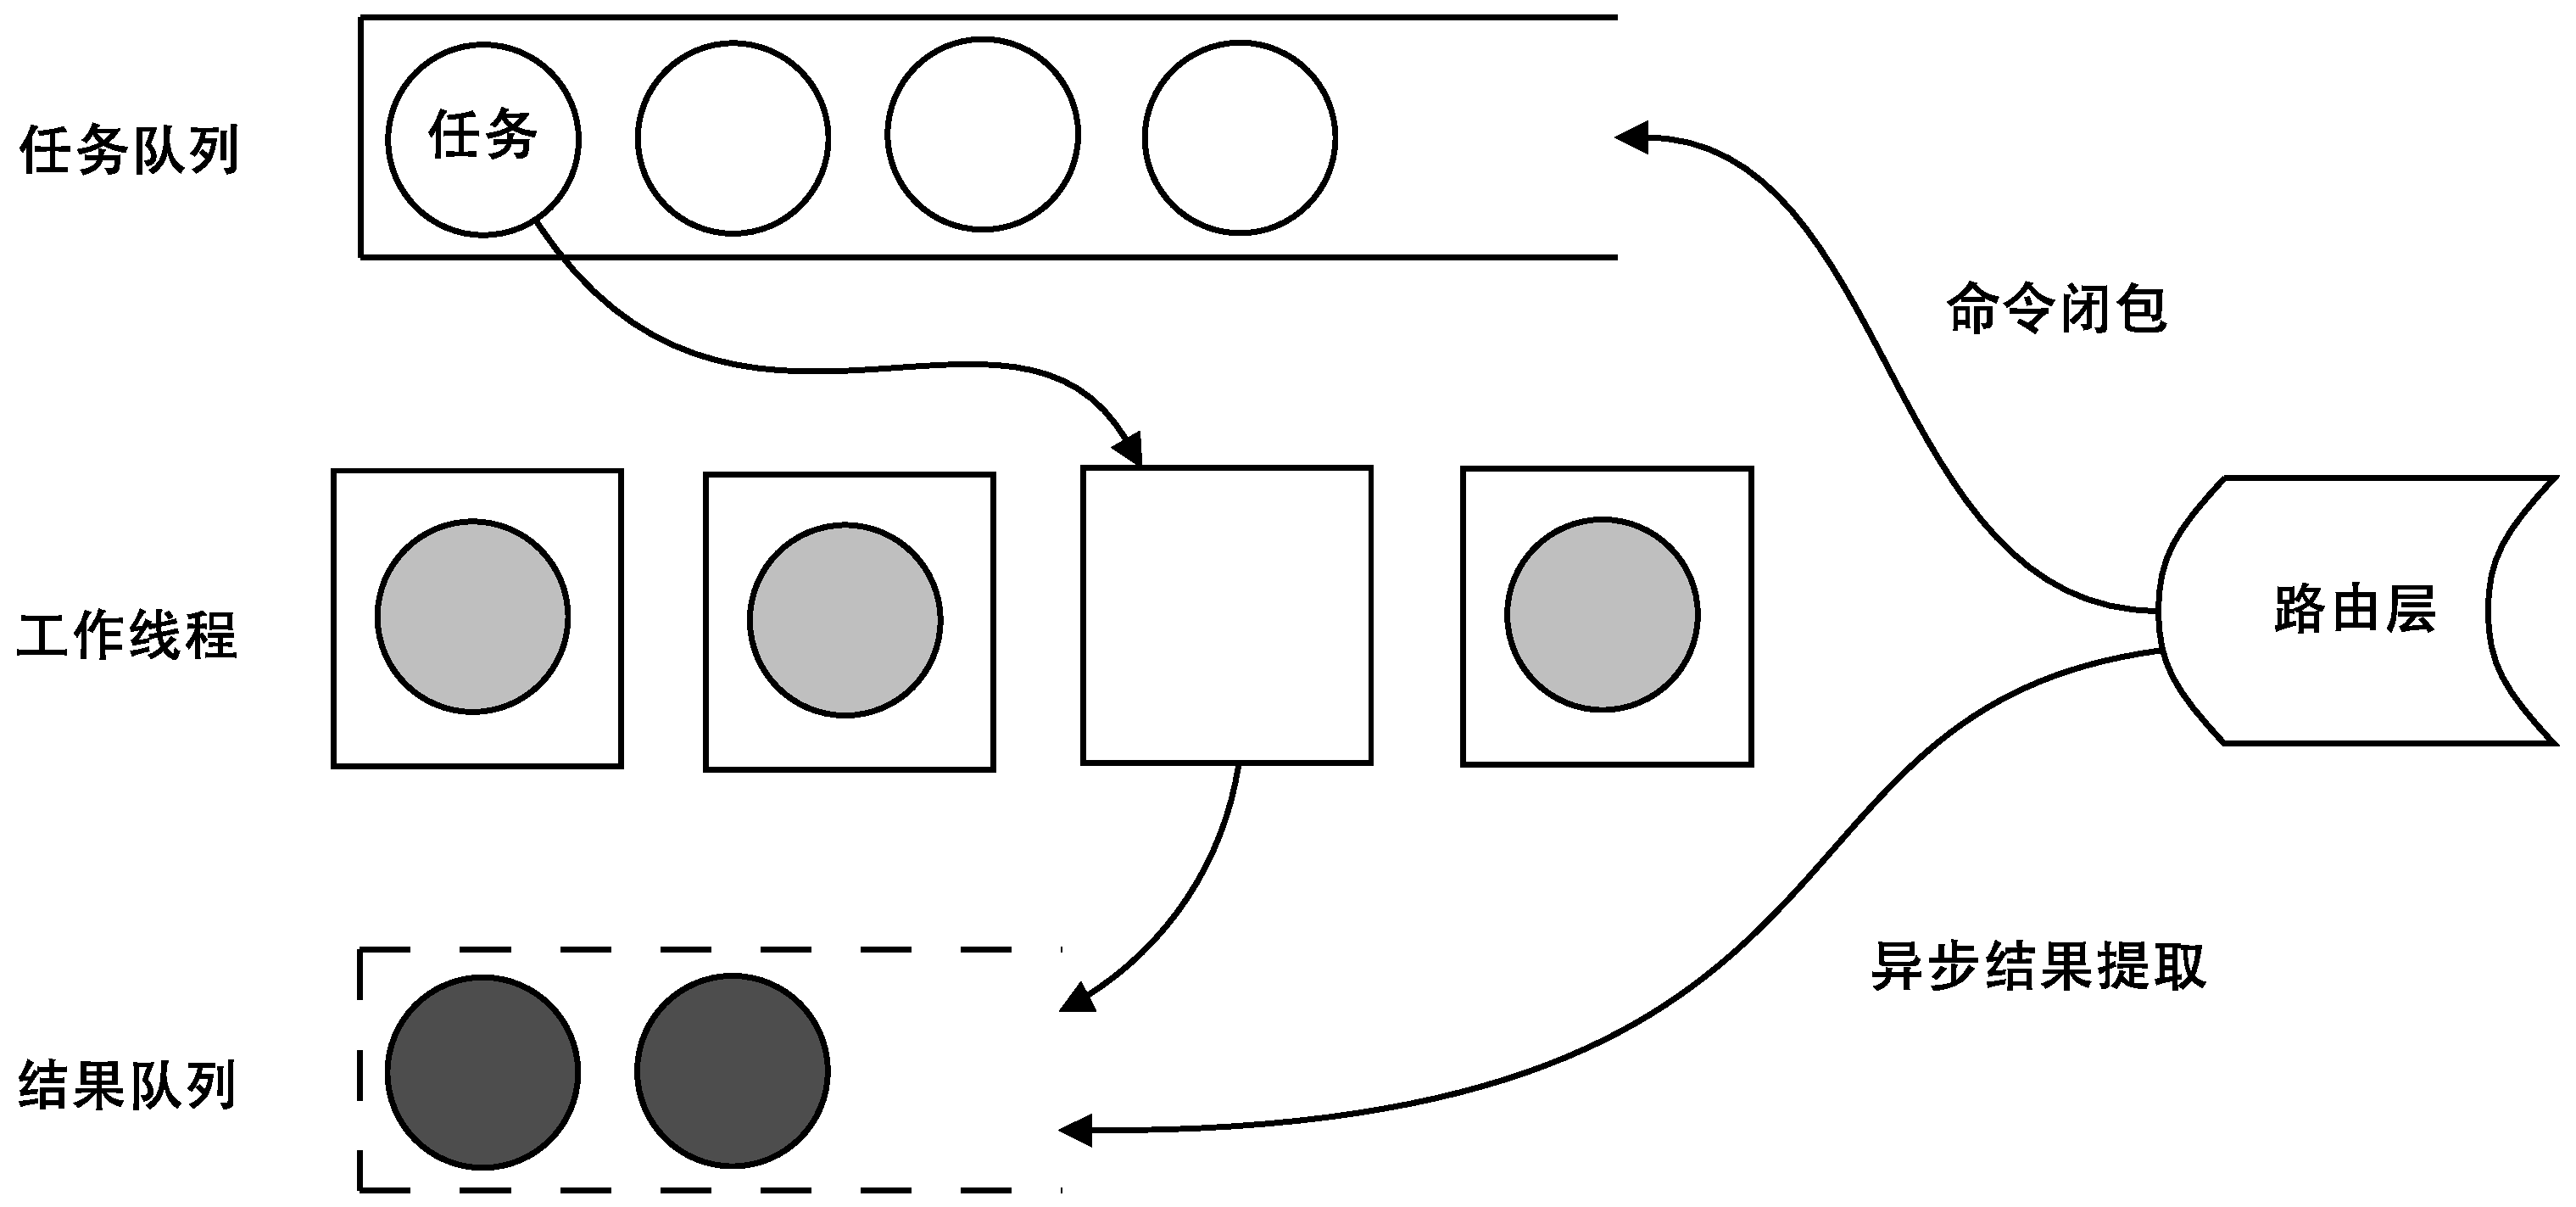
\includegraphics[width=1.0\linewidth]{threadpool}
  \caption[分布式二级哈希表客户端线程池]{分布式二级哈希表客户端线程池工作原
  理。线程池将路由层丢入的命令闭包包装成任务丢入任务队列。空闲的工作线程自动执
  行排在队列中的任务,并将其从任务队列中移出。执行完毕后,该工作线程重新进入空
  闲状态准备执行下个任务。路由层会在一定时限内异步检测命令闭包的执行情况,并从
  中提取结果。}
  \label{figure:threadpool}
\end{figure}

由于工作线程是在线程池初始化的时候创建的,因此当系统饱和运转时,不会有线程创建
和回收资源的开销。不过C语言的标准库中没有线程池的实现,因此我自己利用互斥锁和
条件变量实现了一个高效的线程池。
\begin{code}
typedef struct ThreadPool {
  struct ThreadTask *taskQueue;
  pthread_mutex_t *lock;
  pthread_cond_t *cond;
  pthread_t *threads;
} ThreadPool;
\end{code}
其中,taskQueue是一个用链表实现的任务队列。当路由层请求执行某个命令闭包时,线
程池相应的会创建N个任务,并把它们加入到任务队列的末尾。lock是线程同步互斥锁,
用于保证对线程池结构体任何操作的原子性。cond是线程条件变量,它与lock一起,用于
通知空闲的工作线程任务队列里有等待被执行的任务,实现任务对工作线程的分配。
threads是工作线程,这些线程在线程池初始化的时候创建,之后每个线程进入忙等
\footnote{http://en.wikipedia.org/wiki/Busy\_waiting}循环。在这个循环的一开
始,该工作线程阻塞在pthread\_cond\_wait,进入休眠状态并等待条件变量被触发。起
初任务队列为空,一旦有新的任务加入,线程池会触发条件变量。这个时候,某个处于休
眠状态的工作线程被唤醒,将该任务从任务队列中移出,然后判断这时任务队列中是否还
有等待被执行的任务,如果队列不为空,它再触发一次条件变量,最后执行刚刚从任务队
列中取出的任务。线程池实现了任务的异步执行,保证了系统的运行效率,主要体现在:
\begin{enumerate}
  \item 所有工作线程在线程池初始化的时候被创建。当系统稳定运行之后,不存在因为
  线程创建和资源回收带来的开销,系统性能不会受到影响。
  \item 空闲的工作线程取得某个等待被执行的任务之后:
  \begin{enumerate}
    \item\label{item:1} 将其从任务队列中移除。
    \item\label{item:2} 判断此时任务队列是否为空,如果仍然有任务等待被执行,再
    次触发条件变量。
    \item\label{item:3} 执行\ref{item:1}中从任务队列移除的任务。
  \end{enumerate}
  这三步必须按顺序执行。\ref{item:1}在\ref{item:2}之前保证了所有任务都会被执
  行,而且同一个任务只能被一个工作线程执行。\ref{item:2}在\ref{item:3}之前则
  使得任务可以被并行执行,保证了系统的运行效率。
\end{enumerate}

\subsubsection{命令闭包}
在分布式二级哈希表中,命令闭包是这样一个结构体,它包含一个操作的全部信息。
\begin{code}
typedef struct RedisCommand {
  int (*command) (void *);
  char *key;
  char *field;
  void *value;
  int successNum;
  int exist;
  void *blob;
  pthread_mutex_t *lock;
  int refNum;
} RedisCommand;
\end{code}
其中,command函数指针是将要被工作线程执行的例程,上层应用调用接口层的某一函数
时,路由层根据其语义选择一条Redis命令来实现,即为该函数指针所指向的函数。key,
field, value三个指针分别指向对应数据的两级索引和内容,如果不涉及则为NULL。由于
该命令闭包对应的操作将要在N个副本上执行,因此successNum用于存放成功操作的计
数。exist专门用于表示桶或blob是否存在。假设每个blob的最大长度为L字节,对于读取
blob操作,blob指针用于存放返回值,它指向一块大小为$N * L$的已经申请的内存空
间,第i个完成该操作的工作线程将读取的结果填放在起始地址为$blob + (i - 1) * L$
的内存空间中。lock是该命令闭包的同步互斥锁,用于保证计数等操作正确执行。

\subsubsection{任务}
在分布式二级哈希表中,任务是这样一个结构体,它是任务队列中的元素,可以被任何一
个工作线程执行。
\begin{code}
typedef struct ThreadTask {
  RedisCommand *redisCommand;
  struct in_addr *ip;
  struct ThreadTask *next;
} ThreadTask;
\end{code}
对于上层应用的每个请求,路由层都会创建一个命令闭包,该操作将分别在N个副本上并
行执行,因此线程池将为每个命令闭包创建N个任务。这N个任务的redisCommand指针都指
向这个命令闭包。同时,路由层从配置服务器获取到的N个目标存储服务器的IP地址也将
被分配到这些任务中去。这样,每个任务结构体就包含了执行任何一个请求所需要的全部
信息。

\subsubsection{异步结果提取}
线程池实现了操作的异步化,也使得路由层需要定期查看命令闭包的执行情况。路由层会
在一定时限内以一定频率不断检查命令闭包的successNum域,如果按照$R+W>N$语义达到
了指定的数值,该操作被认为执行成功。如果有返回值,则按照上文提到的方法提取返回
值。由于结果提取可能在N个操作都成功执行之后,也可能在没有全部执行之后,因此需
要某种机制来保证命令闭包在结果提取之后再进行资源回收。在分布式二级哈希表中,这
通过命令闭包结构体的引用计数域refNum实现。该域在命令闭包创建时初始化为1。之后
线程池将创建N个任务结构体,每当有一个任务指向该命令闭包,这个命令闭包的refNum
域加1。这样,在这些任务被执行之前,它们所包含的命令闭包的引用计数达到$N + 1$。
之后这N个任务并行执行,其间路由层可能异步提取结果。每当一个任务执行完毕,命令
闭包的引用计数减1;当路由层成功提取了结果,命令闭包的引用计数也减1。一旦命令闭
包的引用计数减至0,该命令闭包结构体的内存资源立即被回收。通过设置命令闭包的引
用计数域,保证路由层在异步提取结果之后,再对其占用的内存资源进行回收。

\subsection{通信层}
通信层是客户端分层结构的最底层,与存储结点上运行的Redis服务器进程交互,传输数
据和指令,完成存储服务器上Redis二级哈希表的本地操作。通信层按照Redis的交互协议
\footnote{http://redis.io/topics/protocol},实现了一些基本Redis命令
\footnote{http://redis.io/commands},通过这些操作来表达分布式二级哈希表接口函
数的语义,其对应关系详见表\ref{table:redis}。
\begin{table}
  \centering
  \caption[分布式二级哈希表使用的Redis命令]{分布式二级哈希表使用的Redis命令。
  客户端的通信层按照Redis规定的交互协议实现了这些基本Redis命令,与存储服务器上
  的Redis服务器进程交互,传输指令和数据,完成存储服务器上Redis二级哈希表的本地
  操作,以表达分布式二级哈希表的语义。}
  \label{table:redis}
  \begin{tabular}{p{2cm}|p{2cm}|p{9.5cm}}
    \toprule[1.5pt]
    \hei 接口函数 & \hei Redis命令 & \hei 说明 \\
    \midrule[1pt]
    createBucket & hSet &
    在本地Redis二级哈希表中存入两级索引分别为bucketID和EXIST\_BLOB\_ID的数据,
    内容为EXIST\_BLOB。其中,EXIST\_BLOB\_ID为分布式二级哈希表设定的一个特殊字
    符串,不会与任何实际数据的blobID相同。\\
    \midrule[1pt]
    deleteBucket & del &
    删除本地Redis二级哈希表中一级索引为bucketID的所有数据。\\
    \midrule[1pt]
    existBucket & exists &
    查看本地Redis二级哈希表中一级索引为bucketID的数据是否存在。\\
    \midrule[1pt]
    deleteBlob & hDel &
    删除本地Redis二级哈希表中两级索引分别为bucketID和blobID的数据。\\
    \midrule[1pt]
    existBlob & hExists &
    查看本地Redis二级哈希表中两级索引分别为bucketID和blobID的数据是否存在。\\
    \midrule[1pt]
    loadBlob & hGet &
    读取本地Redis二级哈希表中两级索引分别为bucketID和blobID的数据。\\
    \midrule[1pt]
    saveBlob & hSet &
    在本地Redis二级哈希表中存入两级索引分别为bucketID和blobID的数据,内容为
    blob。\\
    \bottomrule[1.5pt]
  \end{tabular}
\end{table}

路由层在创建命令闭包的时候,会将其函数指针域指向通信层实现的Redis命令,然后被
线程池中的工作线程所执行。对于某个Redis命令,首先建立到目标存储服务器的socket
连接,然后按照Redis规定的协议向该服务器发送指令和数据,之后在一定的时限之内,
异步读取服务器传回的结果。如果超时没有收到结果,则认为在该存储服务器上的操作失
败。如果成功读到结果,将其填回命令闭包中,路由层会自动从命令闭包读取操作的结果
数据。最后关闭到远端存储服务器的连接。

一次Redis命令的执行包括客户端将指令和数据发送至目标存储服务器,服务器在Redis二
级哈希表上执行本地操作,服务器返回结果。如果出现网络阻塞或者存储服务器负载过重
等情况,从客户端发出请求到服务器返回结果可能经过很长的时间,甚至最终没有结果返
回。如果客户端采用阻塞方式从socket通道读取结果,会严重影响系统性能。为此,客户
端采取异步方式读取结果,在预先设定的时限内,不断的去检测是否有数据传回。如果读
到结果立即返回;如果超时没有读到结果,则认为此次操作失败。因此,时限的设置尤为
关键,时限大则操作成功率较高,但平均响应时间也会增大;反之,时限小则操作成功率
和平均响应时间都会降低。由于在当前的系统实现里,时限的设置实在系统运行之前静态
确定的,因此需要综合考虑第\ref{section:assumption}节中关于系统操作成功率和平均
响应时间的要求,具体的数值设置参见第\ref{chapter:lab}章。

\section{存储服务器}\label{section:redis}
存储服务器是分布式二级哈希表存储集群中的单个结点,是一致性哈希算法中的一个物理
结点,通过IP地址来区分。存储服务器内部的存储称为本地存储,解决的是本机上索引到
数据的映射关系。在第\ref{chapter:architecture}中曾提到过,分布式二级哈希表的本
地存储采用Redis开源项目。分布式二级哈希表的客户端直接与存储服务器上的Redis服务
器进程交互,对存储服务器上的数据进行操作,并获取返回值。Redis是一个增强的哈希
表,其数据可以是哈希,也就是说,Redis实现了单机的二级哈希表。分布式二级哈希表
则通过一致性哈希,将数据以桶为基本单位,在各个存储服务器上进行分配和备份,实现
了表\ref{table:api}罗列的调用接口函数。

本地存储是分布式二级哈希表需要解决的问题之一,它在很大程度上决定了系统的吞吐率
和平均响应时间。不过,分布式存储系统往往更关心数据是如何在存储集群的结点间进行
分配和备份的,而单个结点上的存储方式则使用已经成熟的本地存储技术。这一方面是由
于分布式存储系统和其他的分布式系统一样,呈现给用户的是独立的接口。在上层应用看
来,它在一个分布式存储系统中操作数据和它在一个单独的存储单元上操作数据,在使用
方式上不应该有任何的差别,只是性能有所不同。分布式存储系统只要解决好数据在系统
中多个存储结点上的分配和备份即可,因为组成系统的最小存储单元可能是一台计算机,
也可能是另一个子分布式存储系统。另一方面,为了提高系统的可扩展性,增强系统的普
适性,不应该对系统中单个结点上的本地存储方式提出过多的要求。随着对分布式存储系
统的利用,可用的存储空间越来越小,势必要求系统通过增加存储结点来提高总存储容
量。对组成系统的单个结点的限制越少,那么可以加入系统的结点越多,系统的可扩展性
越强。例如像Google File System\cite{ghemawat2003google}那样的分布式文件系统,
主要解决的是数据如何在不同存储结点上进行分配和备份的问题,以及用户如何能够找到
想要的数据的问题。系统完全没有对单个结点上的文件系统提出任何要求。只要具备可用
的本地文件系统,任何一台计算机,甚至任何一个分布式文件系统,都可以作为一个基本
的存储单元,加入到Google File System集群中去。

在当前的应用假设下,分布式二级哈希表被设计为不支持存储结点的动态加入和移除。但
是实现数据分配和备份采用了一致性哈希算法,使得系统具备很强的扩展潜能。选择一个
已经很成熟的开源项目Redis作为本地存储模块,在保证系统运行效率的同时,也使我将
主要精力投放在改进和优化数据分配和备份上,着重解决那些在分布式存储系统中存在,
而在本地存储系统中不必考虑的问题。

当然,Redis本身是一个非常出色的本地增强哈希表,支持二级哈希表的语义。此外,系
统在用户态实现了一个虚拟内存层,将全部数据放置在内存或者用户态的虚拟内存中,大
大提升了系统的处理速度,降低了操作的平均响应时间。将数据存放在内存中具有一定的
风险,因为一旦断电,内存中的数据就会全部丢失且无法恢复。每经过一段固定的时间,
或者系统中的数据进行了固定次数的更新操作,Redis就会将内存和用户态虚拟内存中的
数据压缩后写入硬盘。此外,Redis还通过日志文件机制
\footnote{http://en.wikipedia.org/wiki/Journaling\_file\_system}将各个操作以日
志的方式记录下来,提高数据的恢复速度,并且保证数据不会丢失。受篇幅限制,本论文
不对Redis做过多讨论,其架构设计和实现细节可以通过阅读Redis的源代码
\footnote{https://github.com/antirez/redis}来深入了解。本节只粗略说明Redis是如
何实现本地二级哈希表存储的。

Redis是用标准C语言写成的。由于C语言的标准库没有哈希表这种数据结构,Redis自己实
现了一个哈希表。与分布式二级哈希表的一致性哈希模块相同,Redis本地哈希表也采用
128位MD5哈希函数。为了解决哈希冲突,Redis中的桶结构用链表实现,在桶内查找元素
直接遍历链表中的元素,复杂度为O(N),其中N为链表长度。在二级哈希表中,数据的类
型又是一级哈希,这一级哈希的映射关系用一个特定格式的字符串表示,称为\emph{哈希
串}。哈希串的结构为:
\begin{center}
$<H><L_1><k_1><I_1><F_1><v_1>\dots<L_N><k_N><I_N><F_N><v_N>$
\end{center}
各子串的含义和编码规则参见表\ref{table:zipmap}。举例来说,如果某个映射关系为
$\left\{foo: bar, hello: world\right\}$,那么表示它的哈希串的一种可能形式为
\textbackslash x02\textbackslash x03foo\textbackslash x03\textbackslash
x00bar\textbackslash x05hello\textbackslash x05\textbackslash
x00world\textbackslash xFF。在二级哈希表中查找元素的复杂度为O(N),其中N为这个
哈希表中元素的的个数。
\begin{table}
  \centering
  \caption[Redis二级哈希表哈希串结构]{Redis二级哈希表哈希串结构。哈希串是多个
  子串的顺序连接。所有的\emph{长度}均以字节为单位。}
  \label{table:zipmap}
  \begin{tabular}{p{1.5cm}|p{1cm}|p{2.5cm}|p{8cm}}
    \toprule[1.5pt]
    \hei 子串 & \hei 长度 & \hei 含义 & \hei 说明 \\
    \midrule[1pt]
    $<H>$ & 1 & 哈希串长度 & 当数值大于或等于254时,该值忽略。\\
    \midrule[1pt]
    $<L_i>$ & 1或5 & 第i个数据的索引长度 & 把第一字节当作无符号整数。如果小于
    或等于252,此数表示索引长度,该子串长度为1;如果等于253,该子串长度为5,后
    面4字节表示的无符号整数为索引长度;如果等于254,这个位置可以插入新的数据
    (原数据可能由于删除操作被清空);如果等于255,说明这是哈希串的最后一个字
    节。\\
    \midrule[1pt]
    $<k_i>$ & & 第i个数据的索引 & \\
    \midrule[1pt]
    $<I_i>$ & 1或5 & 第i个数据的长度 & 同$<L_i>$。\\
    \midrule[1pt]
    $<F_i>$ & 1 & $<v_i>$之后的无效字节数 & 可能由于更新操作使$v_i$长度变短。\\
    \midrule[1pt]
    $<v_i>$ & & 第i个数据 & \\
    \bottomrule[1.5pt]
  \end{tabular}
\end{table}
